\refstepcounter{figure}
\noindent Figure \thefigure\ shows the packet delivery ratio variation.

\begin{center}
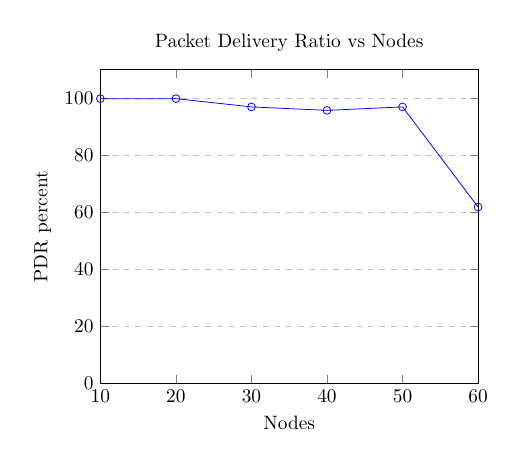
\begin{tikzpicture}[scale=0.7]
\begin{axis}[
title={Packet Delivery Ratio vs Nodes},
xlabel={Nodes}, ylabel={PDR percent},
xmin=10, xmax=60, ymin=0, ymax=110,
xtick={10,20,30,40,50,60},
ymajorgrids=true, grid style=dashed,
]

\addplot[color=blue, mark=o] coordinates {(10,99.89) (20,99.89) (30,97.00) (40,95.78) (50,97.00) (60,61.89)};

\end{axis}
\end{tikzpicture}

\textbf{Figure \thefigure: Packet Delivery Ratio vs Nodes}
\label{fig:pdr_density}
\end{center}